 %\documentclass[handout]{beamer}
%\documentclass{beamer}
\documentclass[aspectratio=169]{beamer}



\usepackage [latin1] {inputenc}		% LaTeX, comprends les accents !
\usepackage [T1] {fontenc}      		% Police contenant les caractères français
\usepackage {geometry}         		% Définir les marges
\usepackage [english] {babel}  	
%\usepackage[backend=biber]{biblatex}
%\bibliography{bib.bib}
\setbeamertemplate{bibliography item}[text]
\usepackage{color}
\usepackage{wasysym}
\usepackage{xcolor}
\usepackage{cancel}
\usepackage{fancybox}
\usepackage{changepage}
\usepackage{tcolorbox}


\usepackage[export]{adjustbox}
\usepackage{tabulary}
\newcolumntype{K}[1]{>{\centering\arraybackslash}p{#1}}

\usepackage{booktabs}
\usepackage{multirow}
\usepackage{fixltx2e}

\usepackage{fancyvrb}
\usepackage {graphicx}
\usepackage{url}
\usepackage {amsmath}
\usepackage {array}
\usepackage {tikz}
\usepackage{pgfkeys}
\usetikzlibrary{shapes,arrows}
\usepackage {subfigure}												% Pour les subfigures
\usepackage{enumitem}
\usepackage{bm}

\usepackage{algorithm}
\usepackage{algpseudocode}
\usepackage{caption} % For caption*
\usepackage{fontawesome}


%\usepackage{eso-pic}    % Pour ajouter des éléments en arrière-plan

%\setlist[itemize,1]{label=$\times$}%
%\setlist[itemize,2]{label=$\checkmark$}
\setlist[itemize,1]{label=$\diamond$}
\setlist[itemize,2]{label=$-$}

\usepackage{listings} 
%\usepackage{color}

\definecolor{mygreen}{rgb}{0,0.6,0}
\definecolor{mygray}{rgb}{0.5,0.5,0.5}
\definecolor{mymauve}{rgb}{0.58,0,0.82}

\lstset{ %
backgroundcolor=\color{white},   % choose the background color; you must add \usepackage{color} or \usepackage{xcolor}; should come as last argument
basicstyle=\footnotesize,        % the size of the fonts that are used for the code
breakatwhitespace=false,         % sets if automatic breaks should only happen at whitespace
breaklines=true,                 % sets automatic line breaking
captionpos=b,                    % sets the caption-position to bottom
commentstyle=\color{mygreen},    % comment style
deletekeywords={...},            % if you want to delete keywords from the given language
escapeinside={\%*}{*)},          % if you want to add LaTeX within your code
extendedchars=true,              % lets you use non-ASCII characters; for 8-bits encodings only, does not work with UTF-8
frame=single,	                   % adds a frame around the code
keepspaces=true,                 % keeps spaces in text, useful for keeping indentation of code (possibly needs columns=flexible)
keywordstyle=\color{blue},       % keyword style
language=Octave,                 % the language of the code
morekeywords={*,...},           % if you want to add more keywords to the set
numbers=left,                    % where to put the line-numbers; possible values are (none, left, right)
numbersep=5pt,                   % how far the line-numbers are from the code
numberstyle=\tiny\color{mygray}, % the style that is used for the line-numbers
rulecolor=\color{black},         % if not set, the frame-color may be changed on line-breaks within not-black text (e.g. comments (green here))
showspaces=false,                % show spaces everywhere adding particular underscores; it overrides 'showstringspaces'
showstringspaces=false,          % underline spaces within strings only
showtabs=false,                  % show tabs within strings adding particular underscores
stepnumber=1,                    % the step between two line-numbers. If it's 1, each line will be numbered
stringstyle=\color{mymauve},     % string literal style
tabsize=2,	                   % sets default tabsize to 2 spaces
title=\lstname                   % show the filename of files included with \lstinputlisting; also try caption instead of title
}

%\setbeamersize{text margin left=1.5cm} 
\definecolor{HardTitle}{RGB}{50,50,160}
\definecolor{LightT}{RGB}{0,0,255}
\definecolor{cadmiumgreen}{rgb}{0.0, 0.42, 0.24}
\beamerboxesdeclarecolorscheme{clair}{LightT}{white}
\usetheme[]{default}

\usecolortheme{default}
%\setbeamercolor{frametitle}{fg=HardTitle, bg=white}
\useinnertheme{default}
\useoutertheme{default}
\setbeamertemplate{footline}{\begin{flushright} \insertframenumber \hspace*{0.5cm} \end{flushright} }
\setbeamertemplate{navigation symbols}{}

\setbeamertemplate{itemize item}{\textbullet}
\setbeamertemplate{itemize subitem}{\textbullet}


%%%%%%%%%%%%%%%%%%% PLOTS
\usepackage{pgfplots}
%\usetikzlibrary{external}
%\tikzexternalize[prefix=Numerical_results/]
\pgfplotsset{compat=1.13}


\tikzstyle{loosely dashed}=          [dash pattern=on 3pt off 6pt]
\pgfplotsset{plotOptions/.style={%
%		y post scale=0.8,
%		ymin=0,ymax=100,
%		ymin=0,
%		xmin=0,xmax=100,
%xlabel={Iteration counter $k$},
%ylabel={$f(x_k)-f(x_\star)$},
%label style={font=},
%legend style={font=},
%		legend pos=north west,
%		legend cell align=left,
%yticklabels=\empty,
%xticklabels=\empty,
%tick label style={font=},
%		no markers,
solid,
very thick
}}
\pgfplotsset{plotOptions2/.style={%
		%		y post scale=0.8,
		%		ymin=0,ymax=100,
		%		ymin=0,
		%		xmin=0,xmax=100,
		xlabel={Lipschitz constant $L$},
		ylabel={Contraction rate $\rho^2$},
		label style={font=\tiny},
		legend style={font=\tiny},
		%		legend pos=north west,
		%		legend cell align=left,
		%yticklabels={0,1},
		%xticklabels={0,1},
		tick label style={font=\tiny},
		%		no markers,
		solid,
		very thick
	}}
\pgfplotsset{plotOptions3/.style={%
		%		y post scale=0.8,
		%		ymin=0,ymax=100,
		%		ymin=0,
		%		xmin=0,xmax=100,
		xlabel={Iteration counter $k$},
		ylabel={$f(x_k)-f(x_\star)$},
		label style={font=\tiny},
		legend style={font=\tiny},
		%		legend pos=north west,
		%		legend cell align=left,
		yticklabels=\empty,
		xticklabels=\empty,
		tick label style={font=\tiny},
		%		no markers,
		solid,
		very thick
	}}
\pgfplotsset{plotOptions4/.style={%
		width=\linewidth,
		%		y post scale=0.8,
				ymax=100,ymin=.0000001,
		%		ymin=0,
				xmin=0,xmax=50,
		xlabel={Iteration $N$},
		ylabel={$\frac{f(x_N)-f_\star}{\|x_0-x_\star\|^2}$},
		%		ylabel={Evaluations to convergence},
		label style={font=\small},
		legend style={font=\small},
		%		legend pos=north west,
		%		legend cell align=left,
		ytick={10,.001,.0000001},
		xtick={0,10,20,30,40,50},
		tick label style={font=\small},
		%		no markers,
		solid,
		very thick
	}}
	\pgfplotsset{plotOptions5/.style={%
			width=\linewidth,
			%		y post scale=0.8,
			ymax=10,ymin=.00001,
			%		ymin=0,
			xmin=0,xmax=50,
			%		ymin=0,ymax=100,
			%		ymin=0,
			%		xmin=0,xmax=100,
			xlabel={Iteration $N$},
			ylabel={$\frac{f(x_N)-f_\star}{f(x_0)-f_\star}$},
			%		ylabel={Evaluations to convergence},
			label style={font=\small},
			legend style={font=\small},
			%		legend pos=north west,
			%		legend cell align=left,
			%xtick={1,10,100},
			tick label style={font=\small},
			ytick={1,.01,.0001},
			xtick={0,10,20,30,40,50},
			%		no markers,
			solid,
			very thick
		}}	
	
	\pgfplotsset{plotOptionsNeutral/.style={%
			%		y post scale=0.8,
			%		ymin=0,ymax=100,
			%		ymin=0,
			%		xmin=0,xmax=100,
			xlabel={``Time''},
			ylabel={``Error''},
			label style={font=\small},
			%		legend style={font=\tiny},
			%		legend pos=north west,
			%		legend cell align=left,
			yticklabels={},
			xticklabels={},
			%		tick label style={font=\tiny},
			%		xtick label style={no markers},
			%		ytick label style={no markers},
			solid,
			very thick
	}}
%%%%%%%%%%%%%%%%%%%%%%%%%%%
%%%%%%%%%%%%%%%%%%%%%%%%%%% COLORS


\definecolor{silver}{cmyk}{0,0,0,0.3}
\definecolor{yellow}{cmyk}{0,.5,.3,0}
\definecolor{orange}{cmyk}{0,0.5,1,0}
\definecolor{red}{cmyk}{0,1,1,0}
\definecolor{reddishyellow}{cmyk}{0.5,0.2,0,0}
\definecolor{black}{cmyk}{0,0,0.0,1.0}
\definecolor{darkYellow}{cmyk}{0.8,0,0.0,0.5}
\definecolor{darkSilver}{cmyk}{0,0,0,0.1}

\definecolor{lightyellow}{cmyk}{0.0,0,0,0.0}
\definecolor{lighteryellow}{cmyk}{0,0,0.0,0.0}
\definecolor{lighteryellow}{cmyk}{0,0,0.0,0.0}
\definecolor{lightestyellow}{cmyk}{0.0,0,0.0,0.0}

\definecolor{colorP1}{RGB}{55,126,184}  % blue
\definecolor{colorP2}{RGB}{228,26,28}  % red
\definecolor{colorP3}{RGB}{152,78,163} % purple
\definecolor{colorP4}{RGB}{77,175,74}  % green
\definecolor{colorP5}{rgb}{0.6, 0.4, 0.08} % golden yellow
%%%%%%%%%%%%%%%%%%%%%%%%%%%
\makeatletter
\pgfplotsset{
every axis x label/.append style={
alias=current axis xlabel,
},
legend pos/outer south/.style={
/pgfplots/legend style={
	at={%
		(%
		\@ifundefined{pgf@sh@ns@current axis xlabel}%
		{xticklabel cs:0.5}%
		{current axis xlabel.south}%
		)%
	},
	anchor=north
},
},
}
\makeatother
%%%%%%%%%%%%%%%%%%%%%%%%%%%
\definecolor{mycolorOne}{RGB}{255,0,0}
\definecolor{mycolorTwo}{RGB}{0,157,255}
\definecolor{mycolorThree}{RGB}{204,201,0}
\definecolor{mycolorFour}{RGB}{237,127,16}

\definecolor{darkcandyapplered}{rgb}{0.64, 0.0, 0.0}
\definecolor{darkspringgreen}{rgb}{0.09, 0.45, 0.27}
\definecolor{deepcarrotorange}{rgb}{0.91, 0.41, 0.17}

\newcommand{\norm}[1]{{\left\lVert#1\right\rVert}}
\newcommand{\normpsq}[1]{{\left\lVert#1\right\rVert}^2}
\newcommand{\normsq}[1]{{\left\lVert#1\right\rVert}^2}
\newcommand{\normdsq}[1]{{\left\lVert#1\right\rVert}^2}
\newcommand{\inner}[2]{{\left< #1, #2\right>}}
\newcommand{\argmin}[1]{\underset{#1}{\text{argmin }}}
\newcommand{\argmax}[1]{\underset{#1}{\text{argmax }}}
\newcommand{\maxim}[1]{\underset{#1}{\text{max }}}
\newcommand{\suprem}[1]{\underset{#1}{\text{sup }}}
\newcommand{\minim}[1]{\underset{#1}{\text{min }}}
\newcommand{\goto}[1]{\overset{\mu\rightarrow 0}{\rightarrow}#1}
\newcommand{\prox}[2]{\underset{#1}{\mathrm{prox}\left(#2\right)}}
\newcommand{\real}{\mathbb{R}}
\newcommand{\emphcolor}[1]{\emph{\color{red}#1}}
\newcommand{\cond}{\tfrac{\mu}{L}}
\newcommand{\bc}[1]{{\color{blue}#1}}
\newcommand{\rc}[1]{{\color{red}#1}}
\newcommand{\cc}[1]{{\color{cyan}#1}}
\newcommand{\co}[1]{{\color{orange}#1}}
\newcommand{\defeq}{\overset{\text{(def)}}{=}}

\newcommand{\hilbert}{\mathcal{H}}
\DeclareMathOperator{\dom}{dom}
\DeclareMathOperator{\val}{val}
\DeclareMathOperator{\epi}{epi}
\DeclareMathOperator{\trace}{Tr}
\DeclareMathOperator{\tr}{\trace}
\DeclareMathOperator{\linspan}{span}
\DeclareMathOperator{\rank}{rank}
\DeclareMathOperator{\FmuL}{\mathcal{F}_{\mu,L}}
\usepackage{pifont} 
\author{Adrien Taylor}
\title{}
\institute [] {}\date{\today}

\renewcommand{\leq}{\leqslant}
\renewcommand{\geq}{\geqslant}
\renewcommand{\succeq}{\succcurlyeq}
\renewcommand{\preceq}{\preccurlyeq}


%\setbeamersize{text margin left=5pt,text margin right=25pt}
\setbeamerfont{footnote}{size=\tiny}
\setbeamersize{text margin left=6mm,text margin right=6mm} 
\usepackage{changepage}

\newcommand{\picsizeo}{.13}
\newcommand{\picsizeth}{.09}
\newcommand{\picsizet}{.10}
\definecolor{someBlue}{rgb}{0,0,2}
\definecolor{someOrange}{rgb}{0.9290, 0.6940, 0.1250}
\definecolor{darkgreen}{rgb}{0.0, 0.5, 0.0}
\newcommand{\titleB}[1]{{}|\! #1}
\newcommand{\frtitle}[1]{\frametitle{\titleB{#1}}}
\begin{document}


\begin{frame}
\thispagestyle{empty}
\setcounter{framenumber}{0}
\begin{center}
\textcolor{HardTitle}{\Large{}Performance Estimation Problems (PEPs)\\[.5cm]}
 \textcolor{HardTitle}{Systematic, principled, and computer-aided approaches\\to the analysis and design of first-order optimization algorithms}
\end{center}
\normalsize
\vspace{.7cm}
\begin{center}
\small {{Aymeric Dieuleveut, Adrien Taylor}} \\[.5cm]

\includegraphics[width=.2\linewidth]{Logos/X.png}\hspace{2cm} 
\includegraphics[width=.2\linewidth]{Logos/inr_logo_rouge_pms.eps}\hspace{2cm} 
\includegraphics[width=.2\linewidth]{Logos/logo_ens_psl_couleur.png}\\[1cm]

\scriptsize SMAI-MODE tutorial -- March 2026

\end{center}
\end{frame}


%%(45mins?) Problème primal+dual bébé (exemple?) [par exemple --> je peux faire mon speech usuel "example-based" /// on utilise le fait qu'ils peuvent tout admettre (interpolation, etc)

%% 2. (1h?) Interpolation + Problème primal + dual [cas + général?] --> essentiellement tes slides
%%3. Exercises/exemples & packages [à séléctionner, p-e faire ça pendant 1h en partant du "learning PEPs" // en gros leur faire reformuler des variantes des problèmes déjà vus, p-e un mini-peu de calcul symbolique?] >> on leur fait analyser des algos simples et retrouver des preuves simples d’un bout à l’autre? 1) avec pepit (si on peut avoir le nettoyage de primal et de dual dont les PRs doivent passer, ça serait top non?), et 2) avec Sympy/mathematica, et puis avec PySR, 3) on leur fait écrire la preuve complète (somme d'inégalités et puis reformulation SOS).
%%4. On motive: analyses right, mais… horizon-dependent! On va donc étudier des façons « moins tight » (tight juste sur un petit nombre d’iter) mais qui ne dépendent pas de l’horizon => 1. Cycles (plus facile, non?) et 2. Lyapunov.
%%5. Exos avec Lyapunov et cycles?
%%6. Design methods [Numerically—3 approches: SSEP, convex relaxations, bourrinage] ++ exemples: OgM, Item, silver, opt proximal…?
%%7. Exos de design? (edited)



\begin{frame}\frtitle{Context: numerical (continuous) optimization}\vspace{-1.8cm}
\begin{flushleft}
\begin{tabular}{ll}
\multirow{2}{*}{
\begin{minipage}{.78\textwidth}
\uncover<1->{Minimize $f:\mathbb{R}^d\rightarrow \mathbb{R}$ (e.g., with $f$ continuous)
\[ \uncover<1->{\textcolor{HardTitle}{f(}\textcolor{red}{x_\star}\textcolor{HardTitle}{)}\triangleq}\min_{x\in\mathbb{R}^d} \textcolor{HardTitle}{f(}x\textcolor{HardTitle}{)}.\]\uncover<1->{\textbf{Ubiquitous in applied mathematics and computer science.}}}
\end{minipage}}&
\multirow{2}{*}{
\begin{minipage}{.21\textwidth}
\begin{center}
\alt<1->{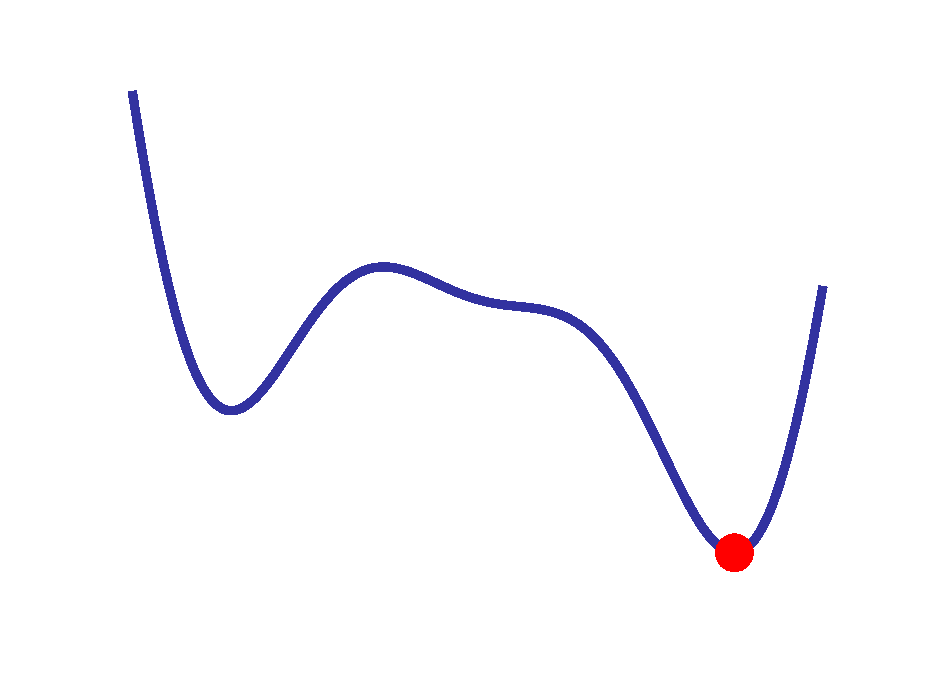
\includegraphics[width=.99\linewidth]{Pics/pretty_example_2.eps}}{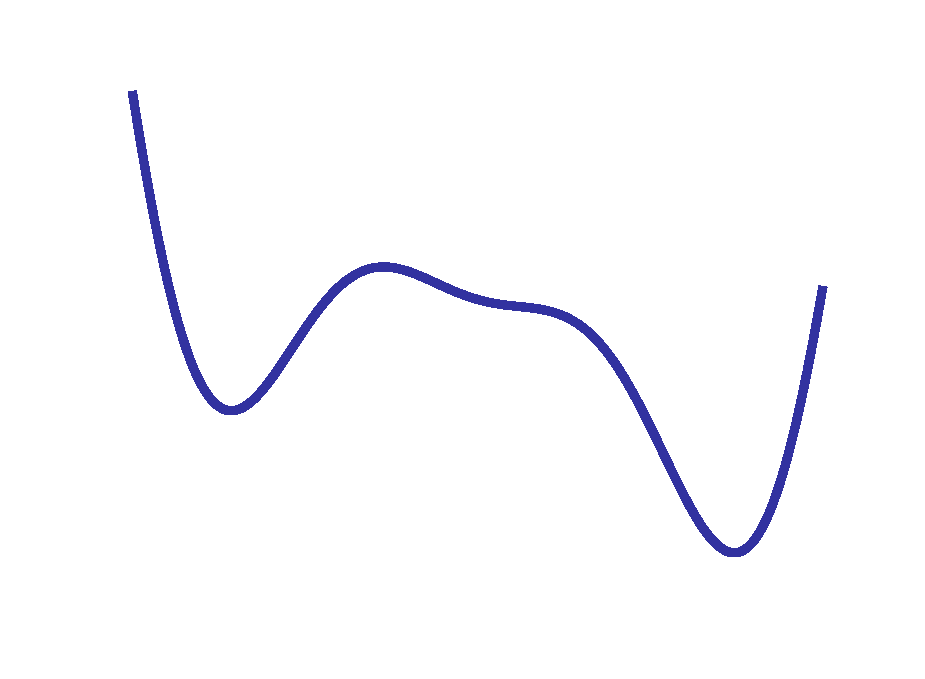
\includegraphics[width=.99\linewidth]{Pics/pretty_example_1.eps}}
\end{center}
\end{minipage}}\\
& \\[1.7cm]
\multicolumn{2}{l}{
\uncover<1->{\hspace{.15cm}\begin{minipage}{\linewidth}
 Numerous applications for modeling (physics, economics), estimation\newline{}(statistics, machine learning), decisions (control, operations research).}
\end{minipage}}\\[.3cm] 
\end{tabular}
\end{flushleft}

\end{frame}


\begin{frame}
\vspace{.2cm}
\small

\uncover<1->{Usually solved via {\bf iterative algorithm} generating sequence $x_0,x_1,\ldots,x_N$.}

\vspace{0.2cm}

\begin{center}
\begin{tabular}{@{}m{0.48\linewidth}@{}m{0.48\linewidth}@{}} % m{} for top alignment
% --- Image column ---
\uncover<1->{
      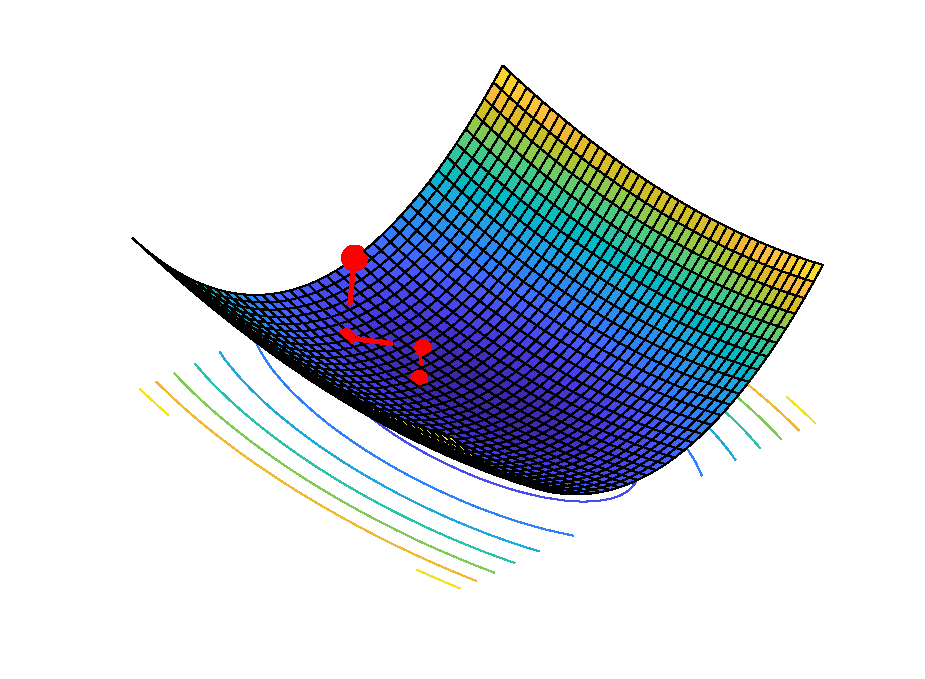
\includegraphics[width=\linewidth]{Pics/gradient_example3.eps}
}%
&\hspace{1cm}
% --- Algorithm column ---
\uncover<1->{%
\begin{minipage}[t]{\linewidth}\vspace{-2cm}
\scriptsize
\alt<3->{\vspace{-.5cm}
\newcommand{\ssu}{3}
\newcommand{\ssd}{4}
\newcommand{\sst}{5}
\newcommand{\ssq}{6}
\newcommand{\ssc}{7}	
\begin{tikzpicture}[scale=.7, transform shape]
				\begin{loglogaxis}[plotOptionsNeutral, ytick=\empty, xtick=\empty,ymin=1e-5, ymax=10,xmin=0,xmax=200,width=.99\linewidth,ylabel style={yshift=4pt,font=\small},xlabel style={yshift=-4pt,font=\small}]			
				\only<{\ssq}->{\addplot[color=mycolorThree,domain=1:100, samples=15,mark=*]{1/x^(2)}};
				\only<{\sst}->{\addplot[color=mycolorTwo,domain=1:55, samples=15,mark=*]{exp(-x/5)/exp(-1/5)}};%, only marks
				\only<{\ssu}->{\addplot[color=mycolorOne,domain=1:100, samples=15, mark=*]{exp(6.5/x)/exp(6.5)}
				};
				\only<{\ssc}->{\addplot[color=mycolorFour,domain=1:100, samples=15, mark=*]{(x/10+1/x^(2))/(1/10+1)}};
				\end{loglogaxis}
				\node[color=mycolorOne] (b1) at (1.4,2.4) {};
				\node[color=mycolorTwo] (b2) at (1.2,3.7) {};
				\node[color=mycolorThree] (b3) at (2.5,2.3) {};
				\node[color=mycolorFour] (b4) at (3,3.9) {};
				
				
				\node[color=mycolorOne] (a1) at (.5,-.9) {\alt<{\ssd}->{Fast, then stall?}{\color{white}Fast, then stall?}};
				\node[color=mycolorTwo] (a2) at (0.5,5) {\alt<{\sst}->{Slow, then fast?}{\color{white}Slow, then fast?}};
				\node[color=mycolorThree] (a3) at (5.5,2.6) {\alt<{\ssq}->{Smoothly improving?}{\color{white}Smoothly improving?}};
				\node[color=mycolorFour] (a4) at (5.8,4.8) {\alt<{\ssc}->{Diverging?}{\color{white}Diverging?}};
				\path[->, very thick, mycolorOne!60]<{\ssd}-> (a1.north) edge [out=90, bend left] (b1);
				\path[->, very thick, mycolorTwo!60]<{\sst}-> (a2.south) edge [ ] (b2);
				\path[->, very thick, mycolorThree!60]<{\ssq}-> (a3.west) edge  [out=90, bend right, in=200] (b3);
				\path[->, very thick, mycolorFour!60]<{\ssc}-> (a4.west) edge  [ bend right, in=250] (b4);
				\end{tikzpicture}}{\begin{tcolorbox}[width=.8\linewidth,colback=gray!20,boxsep=-1mm, arc=2mm,top=2.5mm,bottom=2.3mm,colframe=gray!20]\textbf{Gradient descent} (stepsize $\alpha$)\\[-0.2cm]
\begin{algorithmic}[]
\For{$k = 0, 1, \ldots$}\\
    \State $x_{k+1} = x_k - \alpha \nabla f(x_k)$\\
\EndFor
\end{algorithmic}
\end{tcolorbox}}
\end{minipage}
}%
\end{tabular}
\end{center}

\vspace{0.3cm}

\uncover<2->{What to expect from the output of the algorithm?}

\vspace{0.1cm}

\uncover<2->{For instance: \textbf{bounds} on certain notions of ``error'': $f(x_k)-f(x_\star)$, $\|x_k - x_\star\|$, $\|\nabla f(x_k)\|$, etc.}

\end{frame}


\frame{
\begin{center}
	{\Large{}How to show that an algorithm works?}\pause\\
	\vspace{1cm}
	{\begin{minipage}{.63\linewidth}\small
	\begin{itemize}
		\item<2-> Assumptions (no free lunch).
		\item<3-> Here: worst-case perspective.
	\end{itemize}
\end{minipage}
\begin{minipage}{.35\linewidth}
		\begin{tikzpicture}
    % Define the central formula
    \uncover<4>{\node (img) at (0,0) {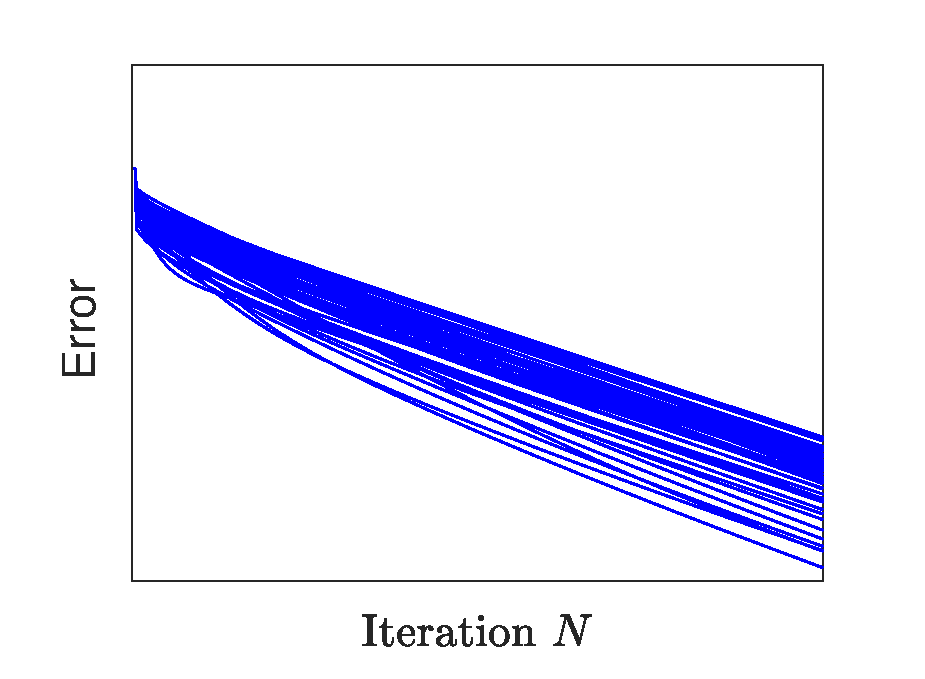
\includegraphics[height=.78\linewidth,width=.99\linewidth]{Pics/quads_GD_colors1.eps}};}
    \uncover<5->{\node (img) at (0,0) {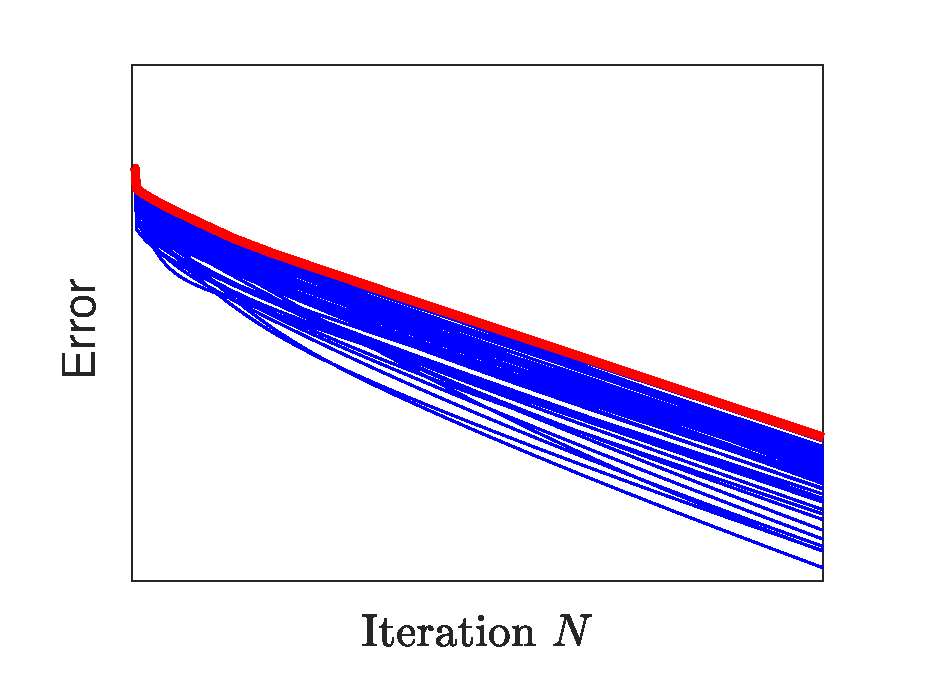
\includegraphics[height=.78\linewidth,width=.99\linewidth]{Pics/quads_GD_colors2.eps}};}
    \uncover<6->{\node (img) at (0,0) {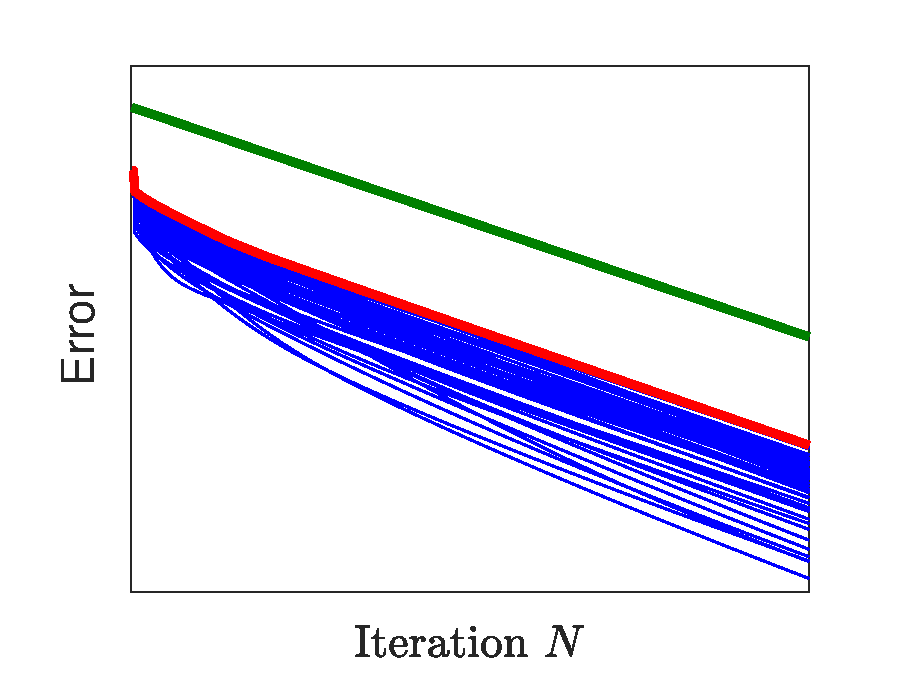
\includegraphics[height=.78\linewidth,width=.99\linewidth]{Pics/quads_GD_colors3.eps}};}
    \uncover<6->{\node [rotate=-20](uu) at (.55,.8) {{\color{darkgreen}upper bound}};}
    \uncover<5->{\node[rotate=-20] (tt) at (0,.4) {\color{red}\text{exact  certificate}};}
    \uncover<4->{\node[rotate=-20] (uu) at (0,-.7) {{\color{someBlue}errors} };}
\end{tikzpicture}
\end{minipage}}
\end{center}	
}

		

\frame{
	\frtitle{Example: analysis of a gradient method }\small
	Let $f:\mathbb{R}^d\rightarrow \mathbb{R}$ (continuously differentiable). Find $x_\star\in\mathbb{R}^d$ such that \begin{align*}f(x_\star)=\min_{x\in \mathbb{R}^d} f(x),\end{align*}
	with $f$ is $L$-smooth and $\mu$-strongly convex ($f\in\mathcal{F}_{\mu,L}$).\\[.6cm]


	\uncover<2->{({Gradient method}) We decide to use: $x_{k+1}=x_k-\alpha  \nabla f(x_k)$}\\[.6cm]
	
	\uncover<3->{{\bf Question}: what \emph{a priori} guarantees after $N$ iterations?}\\[0.3cm]	\begin{itemize}
		\item<3->[]Examples: what about $f(x_N)-f(x_\star)$, $\norm{\nabla  f(x_N)}$, $\norm{x_N-x_\star}$?\\[.6cm]\end{itemize}
	
	
}


\frame{\frtitle{About the assumptions}\small
A differentiable function $f:\mathbb{R}^d\rightarrow \mathbb{R}$ is $\mu$-strongly convex and $L$-smooth iff $\forall x,y\in \mathbb{R}^d$:

\uncover<2->{\begin{center}
				\begin{tikzpicture}[yscale=0.35,xscale=0.35]
				\draw[very thick, black, -stealth] (-10.5,-0.1) -- (11.2,-0.1);
				\draw (11.2,-0.1) node[below left]{$x$};
				\draw[very thick, black, -stealth] (-10,-0.5) -- (-10,8);
				\draw (-10.1,8) node[left]{$f$};
				\draw(0,0) [very thick, color=blue, domain=-3*3:3*3, samples=50] plot({\x}, {2+(\x/4)^2});
				\uncover<3>{\draw(0,0) [dashed,very thick, color=red, domain=-8:0, samples=50] plot({\x}, {2+1-1/2*(\x+4)});}
				\uncover<4->{\draw(0,0) [dashed,very thick, color=red, domain=-8:0, samples=50] plot({\x}, {2+1-1/2*(\x+4)+((\x+4)/5)^2});}
				\uncover<5->{\draw(0,0) [dashed,very thick, color=red, domain=-6.5:-0.7, samples=50] plot({\x}, {2+1-1/2*(\x+4)+1/2*(\x+4)^2});}
				\node [color=red] (poi) at (-4,3) {$\bullet$};
				\end{tikzpicture}
			\end{center}}
			\begin{itemize}
				\item<3->[(1)] (Convexity) $f(x)\geqslant f(y) + \inner{ \nabla f(y)}{x-y}$, \\[0.3cm]
				\item<4->[(1b)] ($\mu$-strong convexity) $f(x) \geqslant f(y) + \inner{ \nabla f(y)}{x-y} +\frac{\mu}{2}\norm{x-y}^2$,\\[0.3cm]
				\item<5->[(2)] (L-smoothness) $f(x) \leqslant f(y) + \inner{\nabla f(y)}{x-y} +\frac{L}{2}\norm{x-y}^2$,\\[0.3cm]
				\item<6->[(1\&{}2)] $\langle{\nabla f(x)-\nabla f(y)};{x-y}\rangle  \geqslant        \tfrac{1}{L+\mu} \lVert{\nabla f(x)-\nabla f(y)}\rVert^2+\tfrac{\mu  L}{L+\mu}\lVert{x-y}\rVert^2$.
				
			\end{itemize}
		}
		
%\frame{assumptions}


%\frame{	\frtitle{Worst-case guarantee for gradient descent?}\scriptsize
%	
%	
%	
%	(Gradient method) For which $C(N,L)$ is
%	\[ f(x_N)-f_\star \leq C(N,L)\,\,{\|x_0-x_\star\|^2}\]
%	true for all $L$-smooth convex $f$ and $x_0\in\mathbb{R}^d$?
%	
%	{Find the worst possible function:
%		\uncover<2->{\begin{align*}
%			C(N,L)=\max_{f,x_0} \ &\frac{ f(x_N)-f_\star}{\|x_0-x_\star\|^2}\\[0.2cm]
%			\text{subject to: } & f \text{ satisfies some assumptions}  & \text{Problem class}\\[0.1cm]
%			&\uncover<2->{x_{k+1}=x_k-\gamma_k \nabla f(x_k) &\text{Algorithm}}\\[0.1cm]
%			\end{align*}}\uncover<3->{Such problem are infinite dimensional (function as a variable).\\[.5cm]}
%	}
%}

%%\frame{\frtitle{Smooth strongly convex functions}
%%	\small {Differentiable function $f:\mathbb{R}^d\rightarrow\mathbb{R}$, $f$ is ($\mu$-strongly) convex and $L$-smooth iff $\forall x,y\in \mathbb{R}^d$ we have:\\[0.3cm]
%%		
%%		\uncover<2->{\begin{center}
%%				\begin{tikzpicture}[yscale=0.35,xscale=0.35]
%%				\draw[very thick, black, -stealth] (-10.5,-0.1) -- (11.2,-0.1);
%%				\draw (11.2,-0.1) node[below left]{$x$};
%%				\draw[very thick, black, -stealth] (-10,-0.5) -- (-10,8);
%%				\draw (-10.1,8) node[left]{$f$};
%%				\draw(0,0) [very thick, color=blue!50, domain=-3*3:3*3, samples=50] plot({\x}, {2+(\x/4)^2});
%%%				\uncover<3>{\draw(0,0) [dashed,very thick, color=red, domain=-8:0, samples=50] plot({\x}, {2+1-1/2*(\x+4)});}
%%				\uncover<3->{\draw(0,0) [dashed,very thick, color=red, domain=-8:0, samples=50] plot({\x}, {2+1-1/2*(\x+4)+((\x+4)/5)^2});}
%%				\uncover<4->{\draw(0,0) [dashed,very thick, color=darkspringgreen, domain=-6.5:-0.7, samples=50] plot({\x}, {2+1-1/2*(\x+4)+1/2*(\x+4)^2});}
%%				\node [color=blue] (poi) at (-4,3) {$\bullet$};
%%				\end{tikzpicture}
%%		\end{center}}
%%		
%%		\begin{itemize}
%%			\item<3->[(1)] \textcolor{red}{($\mu$-strong convexity) $f(x) \geqslant f(y) + \inner{ \nabla f (y)}{x-y} +\frac{\mu}{2}\norm{x-y}^2$,}
%%			\item<4->[(2)] \textcolor{darkspringgreen}{(L-smoothness) $f(x) \leqslant f(y) + \inner{\nabla f (y)}{x-y} +\frac{L}{2}\norm{x-y}^2$.}
%%			
%%		\end{itemize}
%%	}
%%	
%%}


\frame{\frtitle{Convergence rate of a gradient step}\scriptsize
	\vspace{.1cm}
	\uncover<2->{\begin{center}\Ovalbox{ \begin{minipage}{.8\linewidth}\vspace{.3cm}{\bf Toy example}: What is the smallest $\tau$ such that:
					\[ \|x_1-x_\star \|^2 \leqslant \tau \|x_0-x_\star\|^2,\]
					for all
					\begin{itemize}
						\item<3-> $d\in\mathbb{N}$, $L$-smooth and $\mu$-strongly convex function $f$ (notation $f\in\mathcal{F}_{\mu,L}$),
						\item<4-> $x_0$, and $x_1$ generated by gradient step $x_1=x_0-\alpha \nabla f (x_0)$,
						\item<5-> $x_\star=\argmin{x} f(x)$?
	\end{itemize}\end{minipage} }\end{center} }\vspace{.1cm}
	\uncover<6->{
	\begin{equation*}
		\begin{aligned}
		\uncover<6->{\|x_{1}-x_\star\|^2}&\uncover<7->{=\|x_0-x_\star\|^2-2\alpha\langle \nabla f(x_{0});\,x_{0}-x_\star\rangle+\alpha^2\|\nabla f(x_{0})\|^2} \\
		&\uncover<8->{\,\Bigg\downarrow \text{ Inequality (1\&{}2)}} \\
		&\uncover<9->{\leq  \left(1-\tfrac{2\alpha L \mu}{L+\mu}\right)\lVert{x_0-x_\star}\rVert^2+\alpha\left(\alpha-\tfrac2{L+\mu}\right)\lVert{\nabla f(x_0)}\rVert^2}\\
		&\uncover<10->{\,\Bigg\downarrow \text{ if } 0\leq \alpha\leq \tfrac{2}{L+\mu}}\\
		&\uncover<11->{\leq (1-\alpha\mu)^2\|x_0-x_\star\|^2.}
		\end{aligned}
	\end{equation*}}
}

\frame{\frtitle{Convergence rate of a gradient step}\scriptsize
\begin{center}
{\begin{minipage}{.8\linewidth}\small
Legitimate questions:
	\begin{itemize}
		\item<2-> anything improvable? Realistic analyses?
		\item<3-> How to choose the right inequalities to combine? 
		\item<4-> Why studying this specific quantity? Possible to adapt to other quantities?
		\item<5-> Unique way to arrive to the desired result? 
		\item<6-> How likely are we to find such proofs in more complicated cases?
	\end{itemize}
\end{minipage}}
\end{center}
}

\frame{\frtitle{Legitimate questions about performance analyses?}\vspace{-1cm}
\begin{center}
\begin{tabular}{cc}
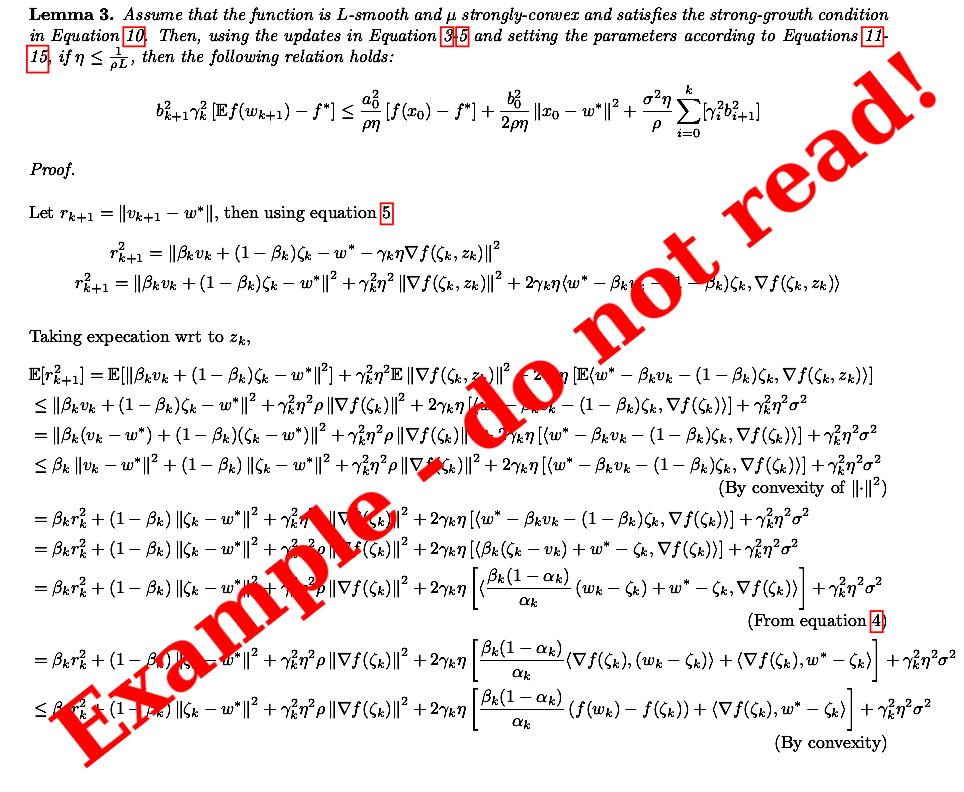
\includegraphics[height=.3\linewidth]{Pics/P1_V4.png} &{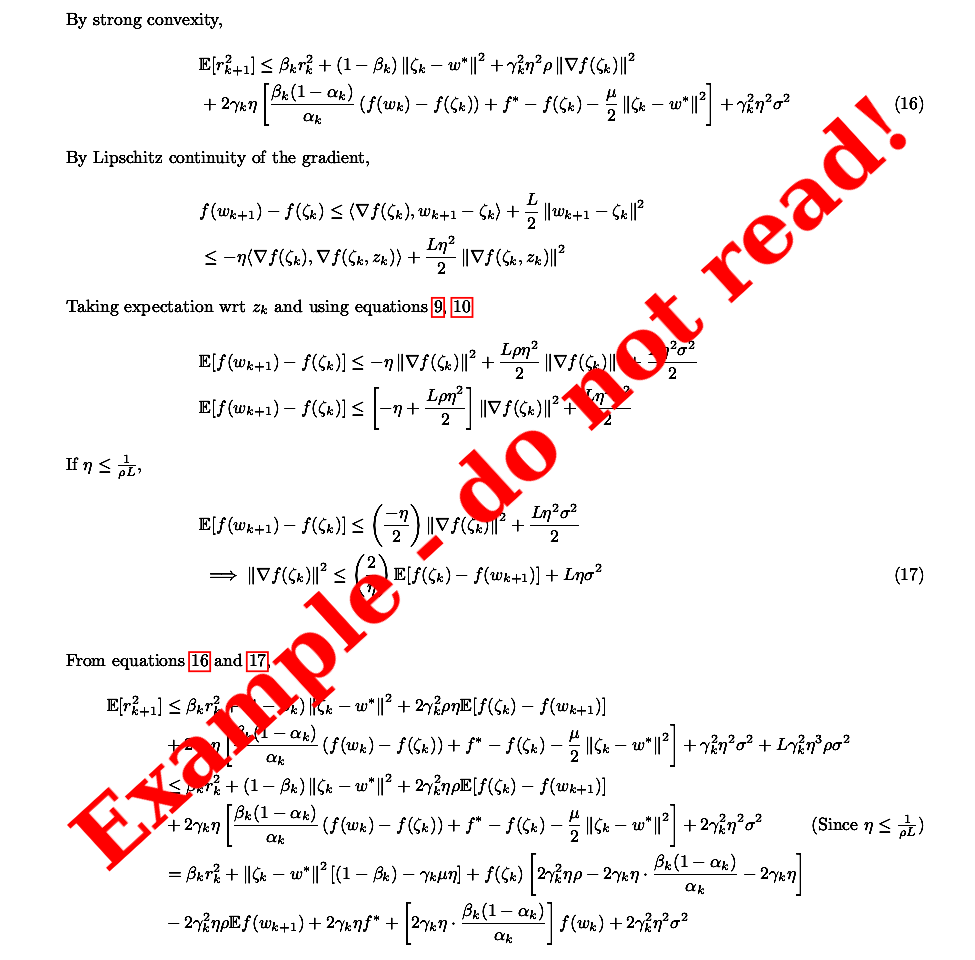
\includegraphics[height=.35\linewidth]{Pics/P2_V3.png}}\\
\end{tabular}
\end{center}
\vspace{-.2cm}
\uncover<2->{
\begin{tcolorbox}[colback=gray!20,width=1.0\textwidth,  arc=2mm,top=.5mm,bottom=.5mm,right=.5mm,left=-.5mm, colframe=gray!20] \normalsize
\begin{tabular}{ll}
\uncover<2->{{\textcolor{red}{\faWarning}} {Error-prone}} & \uncover<2->{{\textcolor{red}{\faQuestionCircleO}} Easily fixable?} \\
\uncover<2->{{\textcolor{red}{\faWarning}} {Technical}, {lack global insights.}} & \uncover<2->{{\textcolor{red}{\faQuestionCircleO}} Simple to adapt to variations of target inequality?} \\
\uncover<2->{{\textcolor{red}{\faWarning}} Few proof patterns.} & \uncover<2->{{\textcolor{red}{\faQuestionCircleO}} Simple to adapt to algorithmic variations?}\\ 
\end{tabular}
\end{tcolorbox}}
\vspace{-2.5cm}

}


\begin{frame}{Organization and learning outcomes (1/3)}

\textbf{Observations:}
\begin{itemize} 
    \item Complexity analyses / convergence proofs for first-order optimization methods often follow very similar (obscure?) patterns.
    \item ... these proofs are rarely intuitive---rely on combining (many) inequalities.
    \item Many variations around same themes.
\end{itemize}

\medskip


\emph{Performance estimation framework}: 
\begin{itemize}
    \item helps understand proof structures of worst-case analyses,
    \item provides principled way to explore complexity bounds/derive such analyses,
    \item mathematical proofs via numerical experiments and symbolic computations.
\end{itemize}

\end{frame}


\begin{frame}{Organization and learning outcomes (2/3)}

\textbf{This mini-course:}

\begin{itemize} 
    \item Interactive introduction to \emph{performance estimation problems}.
    \item Learn how to use numerical PEPs to assess performance of simple first-order algorithms.
    \item Learn how to exploit PEP outputs to construct Lyapunov-based convergence proofs.
    \begin{itemize}
    	\item Sub-goal: construct a proof for a simple gradient-like algorithm.
    \end{itemize}
    \item Symbolic computations for search \& verifying obtained guarantees.
    \begin{itemize}
    	\item Sub-goal: construct a proof for variations around Nesterov's methods.
    \end{itemize}
    \item Learn the basics of PEPs for numerical design of optimization algorithms.
    \begin{itemize}
    	\item Sub-goal: design optimal methods in a few optimization setups.
    \end{itemize}
\end{itemize}

\end{frame}


\begin{frame}{Organization and learning outcomes (3/3)}
\begin{itemize}
    \item[0.] Organization (now) \hfill ($\sim$ 10 mins)
    \item[1.] Motivations, and a full (simple) example \hfill ($\sim$ 60 mins)
    \item[2.] Missing details (and more!):  \hfill ($\sim$ 60 mins)
    \begin{itemize}
    	\item first-order oracles, duality, interpolation,
    	\item semidefinite programming.
    \end{itemize}
    \item[3.] Guided hands-on notebook examples and Q\&A \hfill ($\sim$ 60 mins)
    \item[4.] Compact convergence \& non-convergence certificates \hfill ($\sim$ 90 mins)
    \begin{itemize}
        \item Using PEPs to search for cycles (no convergence).
        \item Using PEPs to search for Lyapunov functions (convergence).
    \end{itemize}
    \item[5.] Guided hands-on notebook examples and Q\&A \hfill ($\sim$ 90 mins)
    \item[6.] Numerical design of optimized algorithms \hfill ($\sim$ 60 mins)
    \item[7.] Guided hands-on notebook examples and Q\&A \hfill ($\sim$ 60 mins)
\end{itemize}
{\color{red}missing 60mins --- 3 blocks (base PEPs, Lyapunov-PEP, design)}
\end{frame}

\begin{frame}{Ressources}

Ressources to be found at
\begin{center}
	\url{https://github.com/PerformanceEstimation/Tutorial-SMAI-MODE}
\end{center}

\medskip
Please:
\begin{itemize}
	\item do interrupt with questions!
	\item We will adapt the pace; program is probably optimistic.
\end{itemize}

\medskip
Tools:
\begin{itemize}
	\item Jupyter notebooks,
	\item Optimization tools/packages
	\begin{itemize}
		\item CVXPY,
		\item if possible: get academic MOSEK license (\url{https://www.mosek.com/products/academic-licenses/})
	\end{itemize}
	\item Symbolics: 
	\begin{itemize}
		\item SymPy
		\item Mathematica is better (but expensive) --- free (limited) version via cloud: \url{https://www.wolframcloud.com/}.
	\end{itemize}
\end{itemize}
\end{frame}
\end{document}


















